% cap2.tex

\chapter{MARCO TEÓRICO}
\label{c2} 


\section{\textit{Cap and Trade} y otros sistemas actuales}\label{c22}
%Agregar desde segundo párrafo de la Revision bibliográfica del hito 1

En el contexto de la generación de energía, el medio ambiente es directamente afectado por la tecnologías utilizadas. Para generar energía se necesita de la combustión de un material, del aprovechamiento mecánico de una energía natural externa u otros como plantas nucleares. Estos sistemas provocan, en distintos niveles y formas, efectos en el medio ambiente. Particularmente las termoeléctricas son consideradas como las que más emisiones de dióxido de carbono producen.
\vspace{2.5mm}

La última importante mención por parte del Gobierno de Chile sobre su plan para combatir esta situación es la propuesta climática a largo plazo \citeB{gobierno_de_chile_estrategia_2021} que Chile presentó en la COP26 el mes de Octubre de 2021. En ella, Chile propone medidas drásticas para combatir las emisiones realizando una propuesta específica en la sección de generación de energía. En ella se presenta un presupuesto límite de emisión de carbono para los generadores de energía. Pero, en contraste, no se incluye un mecanismo o plan específico de como las empresas generadoras lograrán esto y como se llevará a cabo la supervisión de esta meta.
\vspace{2.5mm}

Desde que se reconoció al efecto invernadero como un problema, varios países han comenzado a intervenir, directa o indirectamente, en las industrias que más aportan al efecto. 
\vspace{2.5mm}

Por una parte, el impuesto al carbono o impuesto a emisiones de $CO_2$ consiste en un costo adicional para la generación de electricidad con energías no renovables. El impuesto es cobrado por cada tonelada de este compuesto emitido. Finlandia, en 1990, fue el primer país en implementarlo y desde ahí 18 otros países del continente y muchos otros en el planeta lo fueron implementando a distintos valores por tonelada emitida \citeB{asen_carbon_2021}.
\vspace{2.5mm}

Por otro lado, existen los modelos de \textit{cap and trade}. Concepto creado por Thomas Crocker, consiste en que un ente regulador determina capacidades máximas de contaminación por emisiones a las empresas de la industria eléctrica, donde los emisores son regulados y se les asignan permisos donde si estos superan la capacidad permitida, deben pagar penalizaciones \citeB{hanemann_cap-and-trade_2010}. 
\vspace{2.5mm}

En un contexto donde se busca cumplir con promesas por país para lograr el acuerdo de París (no aumentar la temperatura global en más de 2°C para fines del siglo), un modelo de \textit{cap and trade} es el que parece ser una mejor opción. Esto se debe a que permite establecer, inicialmente, capacidades límites por industria o por país. Entonces, la búsqueda de lograr contaminar un determinado máximo es más creíble que sea realizado con un modelo que regule el contaminante de cada aportante estableciendo una capacidad máxima para ellos. El problema es que cada tipo de \textit{cap and trade} implementado puede afectar en distintas formas la industria, las empresas involucradas y la demanda energética. Por un lado, se puede lograr minimizar emisiones gracias a la reducción en la generación y por otro lado se puede lograr aumentar la cantidad de empresas generadoras con energías renovables.
\vspace{2.5mm}

\citeB{chen_renewable_2021} prueba que aplicar un mecanismo de \textit{cap and trade} es mucho más efectivo en reducir las emisiones de carbono y en incentivar la inversión en energías renovables en comparación con no implementar ningún mecanismo de \textit{cap and trade}. En ese artículo se estudian 3 escenarios aplicados a una empresa monopolística. Los escenarios son: Sin mecanismo de cap-and-trade (NM), con \textit{cap and trade} de regla Grandfathering (GM) y mecanismo de \textit{cap and trade} con regla Benchmarking (BM). El estudio concluye que al implementar mecanismos siempre existirá una mejora en el área de inversión en energías no convencionales o en la reducción en emisiones de carbono. Pero también se concluye que un aumento en la inversión en energías renovables no reduce necesariamente las emisiones de carbono totales, debido a que esta inversión puede ser resultado o respuesta únicamente del aumento en generación y no un reemplazo de generación con un nuevo tipo de origen. Se demuestra que la implementación de BM incentiva más este tipo de inversión mientras que con GM se produce menos emisiones de carbono. De esto es importante destacar que el tipo de mecanismo de \textit{cap and trade} afecta en gran medida el resultado, entonces se debe buscar realizar un modelo que finalmente logre las promesas de contaminación propuestas y no implementar cualquier mecanismo. 
\vspace{2.5mm}

\citeB{wang_impact_2021} se focaliza en el efecto que las implementaciones que los mecanismos \textit{Benchmarking} y \textit{Grandfathering} tienen en las cadenas de suministro de las empresas. Se evalúan como los modelos de financiamiento Bank Credit Financing (BCF) y Trade Credit Financing (TCF), en conjunto con BM y GM, afectan las cadenas de suministro de las empresas y cómo estas se comportan. Se observa el comportamiento de un productor y su proveedor. Finalmente, se concluye que sin importar el mecanismo de \textit{cap and trade}, los productores o fabricantes siempre prefieren BCF mientras que los proveedores se inclinan por TCF. También que el tipo de mecanismo que le convenga al productor dependerá principalmente de sus emisiones históricas.
\vspace{2.5mm}

De estos estudios se entiende la importancia en la implementación del tipo de modelo y de cómo el presupuesto de carbono total puede afectar al mercado. A pesar de que esto, el mismo creador del modelo de \textit{cap and trade}, Thomas Crocker, mencionó en el año 2009 ``Soy escéptico de que un modelo de cap-and-trade sea la forma más eficaz de regular el carbono'' \citeB{yarow_inventor_2009}, debido a que él concluía que era difícil predecir cómo este modelo afectará al mercado de generación en el futuro y si no se tiene un ente regulador eficaz, que fiscalice las emisiones continuamente y establezca las capacidades de forma apropiada, un modelo únicamente con impuesto a la emisión parece ser más eficaz. Por lo que un modelo que se pueda regular solo, en el cual exista incentivo en la disminución de emisión, donde también las empresas generadoras tengan más de una oportunidad para cambiar sus inversiones en capacidad y permisos y que este cambio signifique un beneficio para las empresas, sería un camino apropiado para un modelo de \textit{cap and trade} efectivo. \citeB{amigo_two_2021} propone exactamente esto.


\section{Problemas de equilibrio en capacidad} \label{c21}

Para lograr interpretar la toma de decisiones de los agentes en cualquier sistema es necesario modelar los mecanismos en los cuales están involucrados los diferentes actores. Los modelos de optimización bien diseñados logran orientar la toma de decisiones en base a variables que pueden describir la estrategia de un agente. Estas variables son interpretación de qué decisiones deben tomar los agentes involucrados mientras estos tengan el poder de cambiarlos. 
\vspace{2.5mm}

Un modelo bien estructurado, con restricciones basadas en la teoría económica puede significar un cambio operacional y/o táctico para una empresa. Como también un modelo puede mostrar el comportamiento esperado de un mercado ante variaciones de las estrategias.
\vspace{2.5mm}

Los modelos de equilibrio son aquellos que modelan un problema donde los tomadores de decisión (representados por conjuntos de variables y funciones objetivos en el modelo) cumplen con optimalidad individual y restricciones de equilibrio  asociadas a sus decisiones que relaciones las acciones de todos los agentes involucrados. El concepto de solución del problema está representando por un estado estratégico donde no es posible hacer una acción beneficiosa y todos los recursos han sido asignados a su mejor alternativa sin desperdiciar nada. 
\vspace{2.5mm}

El trabajo \citeB{hu_2_2014}  explica que usando un grupo de ecuaciones matemáticas, se puede explicar el equilibrio que existe entre la oferta y demanda en varios mercados. En ese artículo se explica que el modelo incluye variables endógenas y exógenas para representar el sistema, los cambios en estas últimas logran en las decisiones endógenas al sistema.
\vspace{2.5mm}

Esta memoria concentra el estudio en modelos de equilibrio en capacidad relacionados al mercado de generación eléctrica. Donde existe, por una parte, un equilibrio entre la demanda de energía de los consumidores y la oferta de energía de los productores, y por otra parte, un equilibrio entre la capacidad instalada de los productores y los permisos para emitir contaminantes. Siendo este problema formulado como la minimización anual de inversión en las plantas generadoras de energía.
\vspace{2.5mm}

Los modelos de equilibrio en capacidad han sido históricamente estudiados, como en \citeB{ehrenmann_generation_2011}, \citeB{daertrycke_risk_2017}, \citeB{gabriel_complementarity_2012}, \citeB{ralph_risk_2015}, entre otros.
\vspace{2.5mm}

A continuación, en base al trabajo \citeB{daertrycke_risk_2017}, se explica un problema de equilibrio en capacidad con riesgo asociado de dos etapas y uno de riesgo neutral.

\subsection{Problema de equilibrio en capacidad con riesgo asociado (\textit{risky design equilibrium problem}) y modelos de dos etapas}

En este tipo de problemas existe una variable o vector de variables de diseño denotada como  $x \in \mathbb{R}^{n}$, la cual describe la inversión en activos riesgosos tales como plantas de producción de energía que llevan consigo poderes de producción determinados y proporcionales al grado de inversión en mercados con incertidumbre de demanda.
\vspace{2.5mm}

Es importante entender que estos son problemas de optimización estocásticos. Es decir, existe aleatoriedad respecto a los parámetros de entrada. En este caso, la aleatoriedad se ve reflejada en los escenarios estocásticos posibles con $w \in K$  perteneciente a cada escenario $\{1,...,K\}$ de costos. Entonces, existe una entrada de costos y parámetros $C^{w}$ que corresponden a cada escenario $w$. 

La probabilidad de ocurrencia de cada escenario depende de una distribución de probabilidad $\Theta$, la cuál debe ser definida en el problema estudiado y su implicancia, se ve generalmente, en la notación $E_{\Theta}[Z]$. Esta corresponde a la suma ponderada con una probabilidad de ocurrencia para $z_{w} \in Z$ . En otras palabras, $E_{\Theta}[Z]$ es una suma ponderada del valor de una variable en todos los escenarios multiplicados por la probabilidad de ocurrencia de cada escenario. Para ver un ejemplo de lo anterior, revisar Anexo \ref{ej:sumapond}.

En adición a esto, generalmente, estos modelos tienen dos etapas de decisión $i={0,1}$ para los agentes de producción. Donde en la primera etapa $i=0$ el productor (monopolio) o grupo de productores (mercado competitivo) decide su inversión en capacidad x. Luego, en la segunda etapa $i=1$, se decide la producción Y (recordar que si existe más de un escenario, generalmente escenarios que cambian la demanda o costos, la variable de producción también dependerá del escenario w, teniendo $Y_{w}$ para cada uno).
\vspace{2.5mm}

Como explica \citeB{daertrycke_risk_2017}, estos problemas son, en su forma general, descritos como el siguiente. Donde existe una función $f$ convexa y continua, $g$ convexa y continua donde para cada $x$ :

$$\min f(x,y)\quad\text{sujeta a}\quad g(x,y)\le 0$$

Esto es, se busca minimizar los costos asociados al problema y $g(x,y)$ puede ser una o un grupo de restricciones tecnológicas o de equilibrio del sistema.
\vspace{2.5mm}

Ahora, para contrarrestar los costos asociados a escenarios con incertidumbre, por ejemplo, sub o sobre inversión dependiendo de cada escenario, cada agente $i$ se dota de una medida de riesgo $r_{i}$ que mide su costo de incertidumbre $\Xi_{i}(x_{i},x_{-i})$ como $r_{i}=(\Xi_{i}(x_{i},x_{-i}))$. Esta configuración logra que el agente $i$ tenga que tomar otra decisión de inversión, el agente debe decidir qué productos financieros  $W_i$ perteneciente a $W$ elegir para compensar el riesgo de incertidumbre. Estos productos tienen un precio asociado $P^{\tau}[W]$. Este precio es determinado por la condición de que todos los productos financieros deben balancearse logrando que:

$$\sum_{i=1}^{N}W_{i} = 0$$

Para cada una de las dos etapas de este sistema existen importantes consideraciones.
\vspace{2.5mm}

En la primera etapa, la empresa generadora toma una decisión de inversión en capacidad $x$. 
\vspace{2.5mm}

En la segunda etapa, se sabe la demanda del periodo y la empresa generadora produce de forma costo eficiente. La producción es $Y_{w}$ para el escenario $w$ y se vende la energía a un precio $P_{w}\geq 0$ y costo $C_{w}(Y_{w})$. En cada escenario $w$, la empresa buscará maximizar las utilidades o minimizar los costos de operación y, al mismo tiempo, el demandante buscará maximizar sus utilidades de demanda $Q_{w}$ al comprar la energía al precio $P_{w}$.

\subsection{Caso Riesgo Neutral}

Este es el caso donde todos los agentes involucrados en el problema, determinan o consideran a sus costos estocásticos del problema con la probabilidad $\Theta$ anteriormente explicada de cada escenario $w$. Esto significa que aquellos costos asociados a la producción respetan esta probabilidad pero los costos de inversión en capacidad no son la parte estocástica por lo que no son afectados directamente por esta. En el caso neutro al riesgo existe solamente el riesgo en inversión de capacidad pero no un riesgo de compra de activos financieros ya que los agentes, en este caso, son neutrales al riesgo de intercambio o compra de activos financieros. Este es el caso más estudiado en la literatura en comparación a los de mercados completos e incompletos.
\vspace{2.5mm}

Como se mencionó anteriormente, este estudio explora la aplicación de estos modelos en el mercado de empresas generadoras de electricidad, donde existen dos tipos de agentes, empresas generadoras únicamente de electricidad y demandantes de la energía producida. Este es un caso de mercado competitivo por lo que las empresas no actúan estratégicamente para influenciar los precios. Para todos estos casos en particular, se estudiará la situación donde existen 2 agentes en total, 1 generador de electricidad y 1 demandante. 
\vspace{2.5mm}

Bajo estas circunstancias, se tiene que este es un problema competitivo de equilibrio en capacidad con riesgo neutral si es que existe un grupo de variables $(x_{1}:, Y, x_{2}, Q)$ que resuelva lo siguiente: 

$$ \text{min } I_{1}(x_{1})+ I_{2}(x_{2})+E_{\Theta}[C_{w}(Y_{w}-U_{w}(Q_{w})] (1)$$
$$s.a$$
$$ x_{1} \epsilon X_{1} ,x_{2} \epsilon X_{2}$$
$$A_{1w}x_{1}+B_{1w}Y_{w}+b_{1w} \le 0 $$
$$A_{2w}x_{2}+B_{2w}Y_{w}+b_{2w} \le 0 $$
$$Q_{w}\le e^{\tau}Y_{w}\text{  }\text{ para todo w}$$



\section{MCP y Programación modelos de equilibrio}

\subsection{Resolviendo Problemas de equilibrio mediante MCP}\label{descripcionkkt}

La mayoría de los estudios sobre modelos de equilibrio, ya mencionados anteriormente, explican que la mejor forma para resolver los problemas de este tipo, en especial aquellos con gran cantidad de variables o aquellos no lineales, es transformarlos en problemas de comlementaridad mixta o \textit{Mixed Complementarity Problems} (MCP) en inglés.
\vspace{2.5mm}

\citeB{gabriel_complementarity_2012} explican que para realizar esto en necesario primero estructurar el problema de equilibrio (o cualquiera que cumpla el siguiente estilo) de la siguiente forma:

\begin{align}
    \min_{x} & \quad f(x) \label{foej1}\\ 
    \textrm{s.a.} \nonumber\\
    g_{i}(x) \leq 0 ,\quad & i=1,2,...,n  &(\eta_{i}) \label{resej1} 
\end{align}

Con $f(x)$ función objetivo,  $g_{i}(x):\mathbb{R}^n \rightarrow \mathbb{R}$ restricciones y $\eta_i$ los multiplicadores de Lagrange asociados. 
\vspace{2.5mm}

Puede suceder que las restricciones son con sentido inverso y para eso solo basta con multiplicar la restricción \ref{resej1} por $-1$ y así obtener el sistema de ecuaciones deseado. Si \ref{foej1} es una maximización, basta con multiplicarle $-1$ a la función para convertirla en minimización. Para restricciones con igualdad revisar su metodología en \citeB{gabriel_complementarity_2012}.
\vspace{2.5mm}

Luego, se debe calcular el Lagrangeano de este problema con las variables duales de cada restricción ($\eta_{i}$ en \ref{resej1}) de la siguiente forma:

\begin{align}
    \mathcal{L}=f(x) +  \sum_{i=1}^{n}\eta_{i}g_{i}(x)\label{lagraneanoex}
\end{align}

Finalmente, se puede encontrar un valor óptimo para $x$, donde se cumplan las siguientes condiciones de \textit{Karush-Kuhn-Tucker} (KKT). La primera condición \ref{condicion1}, restringe que el gradiente respecto a la variable $x$ del Lagrangeano en \ref{lagraneanoex} debe ser 0 (estacionariedad). La segunda y tercera condición \ref{condicion2}, \ref{condicion3}, establecen la no negatividad de las restricciones (factibilidad). La última condición \ref{condicion4}, establece la complementariedad entre la restricción y su variable dual respectiva\footnote{\ref{condicion2},\ref{condicion3},\ref{condicion4} pueden ser resumidas en una sola condición como: $0\leq\eta_{i}\perp g_{i}(x)\leq 0$}. 

\begin{align}
    0 = \nabla f(x) + \sum_{i=1}^{n} \eta_{i}\nabla g_{i}(x) \label{condicion1}\\
    -g_{i}(x) \geq 0 &, & i=1,2,...,n  \label{condicion2}\\
    \eta_{i} \geq 0 &, & i=1,2,...,n \label{condicion3}\\
    -g_{i}(x)\cdot \eta_{i} = 0 &, & i=1,2,...,n \label{condicion4}
\end{align}

\subsection{Programando modelos de equilibrio}\label{explisolvers}

A pesar de que existen diversos lenguajes de programación que soportan optimización de modelos y muchos de estos contienen librerías especializadas para encontrar estas soluciones, la utilización de programas que soporten problemas NLP (problemas no lineales) es más conveniente de manejar. Esta sub-sección explica el método de cómputo de modelos de equilibrio NLP en \textit{pyscipopt} (librería soportada por Python), GAMS y MCP en GAMS.

\subsubsection{\textit{pyscipopt}}

SCIP es una librería de código abierto para distintos programas. En su página web oficial, se solicita citar los siguientes 2 artículos \citeB{perron_constraint_2008}
y \citeB{achterberg_scip_2009} al utilizar el \textit{solver} para un trabajo. . 
\vspace{2.5mm}

\textit{Pyscipopt} es la interfaz desde python a la \textit{SCIP Optimization Suite}. La ventaja de este \textit{solver}, en adición a entregar resultados certeros de modelos no lineales, es que presenta la posibilidad de incluir sumatorias propias para definir las restricciones con mayor facilidad y su notación simplifica la posibilidad de incluir variables y de utilizar las funciones usuales de Python sin el cuidado de afectar la sintaxis del solver.
\vspace{2.5mm}

Para utilizar este programa es necesario instalar ciertas interfaces con anterioridad. La forma más rápida y eficiente de poder utilizar esta librería es por medio de Google Colab. Una vez en un archivo Colab, es necesario agregar las siguientes líneas de código:


\begin{lstlisting}[language=Python]
!pip install -q condacolab
import condacolab            
condacolab.install()
!conda install --channel conda-forge pyscipopt
\end{lstlisting}
 
Luego, la codificación del problema a resolver debe seguir la siguiente forma y condiciones:

\begin{enumerate}
    \item Comenzar el modelo: se debe escribir el comienzo del modelo o apertura de su diseño con el siguiente comando,
   \begin{lstlisting}[language=Python]
   modelo=Model()
   \end{lstlisting}
   \item Definir las variables: es necesario definir todas las variables con la siguiente nomenclatura,
   \begin{lstlisting}[language=Python]
   x=modelo.addVar('x', vtype='C')  # C variables continuas 
   y=modelo.addVar('y', vtype='d') # d  variables discretas 
   \end{lstlisting}
   \item Generar la función objetivo: se debe definir la función objetivo de forma directa o a partir de otra variable inventada, acá también se define si el problema es de minimización o maximización,
   \begin{lstlisting}[language=Python]
  modelo.setObjective(x+y, "minimize")
  \end{lstlisting}
  \item Agregar las restricciones: hay que agregar las restricciones del modelo, la naturaleza de las variables se pueden agregar en la misma definición de las variables o como restricción,
  \begin{lstlisting}[language=Python]
  modelo.addCons(x>=y)
  modelo.addCons(x>=0)
  modelo.addCons(y>=0)
  \end{lstlisting}
  
  \item  Resolver el problema: se agrega el comando para que el \textit{solver} optimice y así encuentre la mejor solución posible,
  \begin{lstlisting}[language=Python]
  modelo.optimize()
  \end{lstlisting}
  \item  Llamar a las soluciones encontradas: Este paso no es necesario para resolver el problema pero se necesita si se quieren encontrar las soluciones del problema,
  \begin{lstlisting}[language=Python]
  modelo.getVal(x)
  modelo.getObjVal()
  \end{lstlisting}
\end{enumerate}

\subsubsection{GAMS}

Según lo mencionado en la página de \textit{GAMS Studio}\footnote{\url{https://www.gams.com/34/docs/UG_studio_tutorial.html}}, este es un programa que permite la programación e interfaz gráfica para ejecutar GAMS. GAMS, por su lado, es un lenguaje de programación especializado en resolver modelos de optimización. Este sistema es específico para realizar modelamiento de múltiples tipos de modelos de optimización y con múltiples herramientas para resolverlos. Una de las ventajas de utilizar \emph{GAMS Studio} es el detalle de se entrega luego de encontrada (o no) la solución a un problema de modelamiento. Este detalle demuestra los valores de cada variables en detalle junto con sus intervalos de error posibles y entrega información detallada del computador en el cual se está trabajando. En caso de que el sistema no logre encontrar solución, este entregará esa información junto con posibles problemas del modelo. 
\vspace{2.5mm}

Para utilizar este programa es importante entender el problema de optimización escrito, considerando todas las restricciones del problema y definiendo todas las variables y parámetros adecuadamente. Para que no existan errores, se deben utilizar los separadores como “;” y definir cuales corresponden a variables, escenarios, parámetros, ecuaciones, restricciones y nombrar el modelo. Es importante que al definir las restricciones “=g=” significa “mayor que” , “=l=” significa “menor que” y “=e=” significa “igual que”.

Luego, la codificación del problema a resolver debe seguir la siguiente forma y condiciones:

\begin{enumerate}
   \item Definir las variables: es necesario definir las variables dependiendo de su naturaleza. con la siguiente nomenclatura,
   \begin{lstlisting}
  Positive Variable  x; % se define la variable positiva x
  Binary Variable y; % se define la variable binaria y
  Variable z; % se define la variable real z
   \end{lstlisting}
   \item Se mencionan las ecuaciones del modelo: se deben mencionar todas las ecuaciones del modelo, 
   \begin{lstlisting}
 Equations
 fo funcion objetivo
 rest restriccion;
  \end{lstlisting}
  \item Definir las ecuaciones: después de mencionarlas, hay que definir las ecuaciones del modelo,
  \begin{lstlisting}
  fo.. z=e=5x+2;
  rest.. x=g=0;
  \end{lstlisting}
  
  \item  Definir el modelo y resolver: se define el modelo con las ecuaciones y variables antes definidas, se llama al \textit{solver} con el cuál resolverlo y se define si se debe minimizar o maximizar la función objetivo. 
  \begin{lstlisting}
  Model modelo
  /fo,rest/;
  solve modelo using minlp minimizing z;
  \end{lstlisting}
\end{enumerate}


\subsubsection{GAMS con MCP}

Para programar un problema MCP en GAMS se deben seguir las nomenclaturas mencionadas en la subsección anterior. Con excepción del último punto de definición del modelo y como llamar al solver. 

Primero, es necesario entender que para este estilo de resolución de MCP en \textit{GAMS} es necesario tener el problema listo como un MCP. Para esto, una de las opciones es realizarlo mediante las condiciones de KKT explicadas en \ref{descripcionkkt}. Una vez encontradas las condiciones, se deben utilizar cada una de las derivadas de primer orden del Lagraneano en \ref{condicion1} para despejar las variables duales del problema. Una vez realizado esto, y respetando que se cumple \ref{condicion3}, se puede llamar al \textit{solver} para resolver el problema. 

Por ejemplo, se asume que la \ref{condicion1} de un problema de optimización es el siguiente (con $x$ variable primal y $\eta$ dual):

$$0=x-\eta \leftrightarrow \eta=x$$

Luego, se define la ecuación $kkt$ que corresponde a la dual $\eta$:

\begin{lstlisting}
  kkt.. x=g=0;
 \end{lstlisting}

Finalmente, asumiendo que no hay restricciones adicionales y que la variable x está definida previamente como una variable positiva, se define el modelo y se llama al \textit{solver} \textit{PATH} (para MCPs) de la siguiente forma:

\begin{lstlisting}
  options mcp=path;
  model Modelo2
  /kkt.x/
  solve Modelo2 using mcp;
\end{lstlisting}

Es importante entender que la sección \textbf{/kkt.x/} es la que define la condición de complementariedad \ref{condicion4} del MCP. Siendo \textbf{/kkt.x/} el equivalente a  $kkt \perp x$. 

\subsection{Resolución ejemplo 3.3.1 DÁertrycke et al. (2017)}

Para aplicar lo explicado en la sección \ref{explisolvers}, se lleva a cabo la resolución del problema 3.3.1, presente en la página 24 de \citeB{daertrycke_risk_2017}. Este es un problema competitivo de equilibrio en capacidad con riesgo neutral, el cuál está relacionado con el tema central de este trabajo ya que modela la minimización de costos de generación de electricidad al suplir la demanda energética que esta abastece. 
\vspace{2.5mm}

\subsubsection{Explicación Problema}
En este ejemplo existe un productor, el cuál puede invertir únicamente en una tecnología de producción energética. La planta tiene un costo de capital anualizado $I=90 \frac{\textup{\euro}}{kW}$ y costo de operación $C=60 \frac{\textup{\euro}}{kW}$. El año se representa, para este caso, con duración en horas $\tau = 8760 horas$.
\vspace{2.5mm}

Existen tres variables de decisión en el problema,




\section{Amigo, Cea-Echenique \& Feijoo, 2021}

Como se menciona en \ref{c22}, mecanismos de \textit{cap and trade}, por lo menos en teoría, pueden funcionar de forma efectiva cuando se aplica el método correcto al problema que se quiere solucionar. El modelo de \textit{cap and trade} de dos etapas propuesto por los autores Pía Amigo, Sebastián Cea-Echeñique y Felipe Feijoo en su trabajo titulado \textit{A two stage cap-and-trade model with allowance re-trading and capacity investment: The case of the Chilean NDC targets} busca disminuir las emisiones de $CO_2$ e incentivar el cambio de generación de energía a fuentes más sustentables al aplicar un modelo que reconoce que tanto los productores como el planificador social (subastador o regulador) buscan maximizar sus beneficios.
\vspace{2.5mm}

En él, el modelo propone un sistema de dos etapas involucrando a los generadores de electricidad y al subastador que proporciona los permisos de emisiones de dióxido de carbono ($CO_2 e$). En la primera etapa (periodo $t=0$), el subastador determina los permisos de contaminación que serán vendidos a los productores de electricidad. Estos permisos corresponden a la contaminación máxima que cada generador puede emitir. Por otro lado, en la misma etapa, las empresas generadoras deciden su inversión en capacidad, su generación y la asignación de sus permisos para satisfacer una demanda exógena. Ellos compran los permisos $A_i$ al subastador a un precio $\pi^a$ para poder hacer viable, en términos de permisos de emisión de contaminante, su producción. 
\vspace{2.5mm}

La segunda etapa se distribuye entre el periodo siguiente a la asignación inicial de permisos por parte del subastador hasta el fin del período analizado ($t=1,...,T$). Particularmente en $t=1$ es donde se revela la demanda futura dada por un estado de la naturaleza $w \in W :=\{ 1,..,K\}$ donde su probabilidad de ocurrencia está definida por $P(w)$. Según esta demanda, los productores recalculan sus niveles de generación, determinar nuevamente su capacidad e inversión en permisos faltantes. También tienen la oportunidad de comprar permisos o vender los suyos para adaptar su esperanza de generación en el futuro. Esto les otorga una segunda oportunidad para adaptar sus variables de generación sin ser afectados en gran manera por la incertidumbre de demanda.
\vspace{2.5mm}

\begin{figure}[htp]
    \centering
    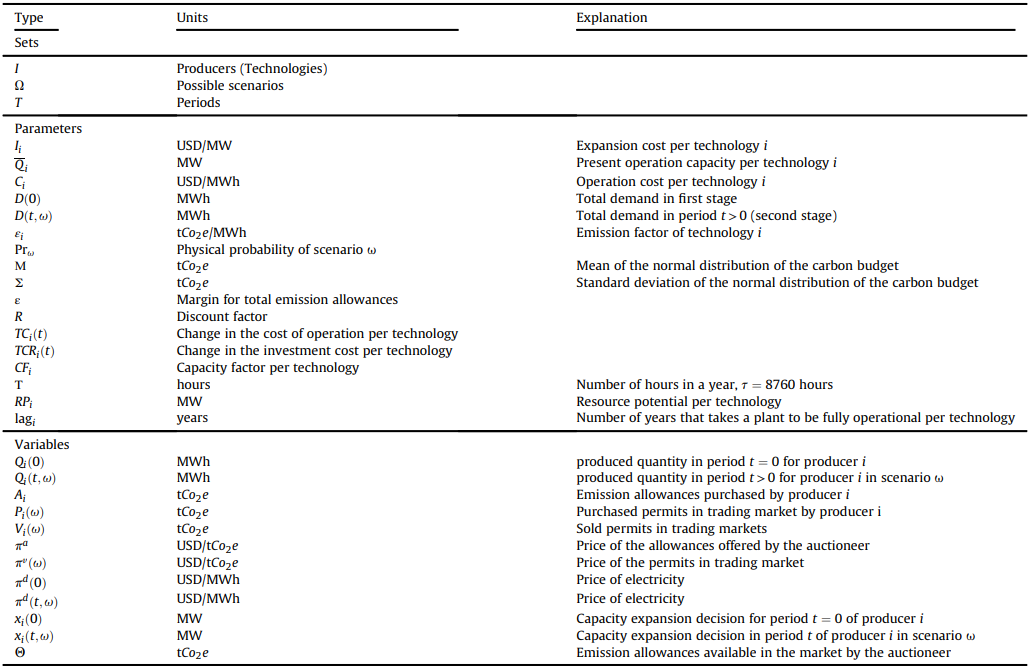
\includegraphics[width=15cm]{docs/DocumentoMemoria/images/Tabla amigo.png}
    \caption{Nomenclatura modelo original (Fuente: \protect\citeB{amigo_two_2021})}
    \label{fig:nomenclatura1}
\end{figure}

La Figura \ref{fig:nomenclatura1} define todas las variables del modelo original para así simplificar la lectura las ecuaciones por definir a continuación.
\vspace{2.5mm}

El modelo completo de \textit{cap and trade} propuesto en el artículo principal es dividido en dos modelos separados de equilibrio en capacidad que modelan el problema de los agentes (subastador y productores) donde ellos buscan maximizar sus beneficios.
\vspace{2.5mm}

Por un lado, está el problema de los productores en \ref{fo:prod}. Esta está acotada por restricciones de capacidad en generación en \ref{res:1}, restricción en generación inicial \ref{res:2}, de limites en capacidad \ref{res:3} y venta y compra de permisos \ref{res:4} y \ref{res:5}. 

\begin{align}
\min_{(x_i,Q_i,A_i,P_i,V_i)\in \mathbb{X}} &  f_i \big( \pi^d(0),Q_i(0)\big)+ A_i \pi^{a} + I_i x_i(0) \nonumber \\ 
& + \sum_{\omega} Pr(\omega)   \Bigg[ \sum_{t>0} \frac{1}{(1+R)^t} \Big[ TC_i(t,\omega)\cdot f_i \big( \pi^d(t,\omega),Q_i(t,\omega) \big)  \nonumber \\
 & + TCR_i(t,\omega) \cdot I_i\cdot x_i(t,\omega) \Big] + \pi^v(\omega)\cdot \big(P_i(\omega)-V_i(\omega)\big) \Bigg]  \label{fo:prod}\\
     \textrm{s.t \ } \nonumber
\end{align}
\begin{align}
    \Big(CF_i \cdot\tau\Big)  \Bigg[\bar{Q}_i + \sum_{t^{\prime}<\bar{t}} x_i(t^\prime,\omega) + x_i(0)+ \bar{Q}_i(t) \Bigg] - Q_i(t,\omega) & \geq 0  & \forall  \quad i,\omega, t  > 0 & \quad (\alpha_{i,\omega,t})\label{res:1}\\
    \Big(CF_i\cdot\tau \Big)\bar{Q_i}-Q_{i}(0) & \geq 0  & \forall  \quad i & \quad (\kappa_i) \label{res:2}\\
     RP_i - \bar{Q}_i  - x_i(0) - \sum_{t > 0} x_i(t,\omega) & \geq 0 &  \forall \quad i,\omega &   \quad (\psi_{i,\omega}) \label{res:3}\\
 A_{i} -V_i(\omega) & \geq  0  & \forall  \quad \omega & \quad (\beta_{i,\omega}) \label{res:4}\\
 A_{i} + (P_i(\omega) - V_i(\omega))-\sum_{t>0}Q_i(t, \omega)\cdot \varepsilon_{i}-Q_i(0)\varepsilon_{i} & \geq  0  &\forall \quad \omega & \quad (\gamma_{i,\omega})\label{res:5}\\
 Q_i(0) & \geq  0 & \forall \quad i & \quad (\lambda_i) \label{res:q0}\\ 
 Q_i(t, \omega) & \geq  0   & \forall \quad \omega, t >0 & \quad (\delta_{i,\omega,t})\label{res:qt}\\
  x_i(0) & \geq  0 & \forall  \quad i & \quad (\xi_i)  \label{res:capi0}\\ 
  x_i(t, \omega) & \geq  0   & \forall  \quad \omega, t >0 & \quad (\varphi_{i,\omega,t})\label{res:capt}
  \end{align}

Es de importancia mencionar que las variables presentes al final de cada restricción (por ejemplo $\varphi_{i,\omega,t}$ en \ref{res:capt}) corresponden a las variables duales de cada una respectivamente.
\vspace{2.5mm}

Por otro lado, el problema del subastador está formulado de la siguiente forma en \ref{eq:sub}. En la sección siguiente se explica con más detalle este modelo y sus restricciones.

\begin{equation}
\begin{array}{rrclcl}
    \displaystyle \min_{\theta} &-\theta \pi^a + F(\theta) \\\textrm{s.a.} \label{eq:sub}\\
\end{array}
\end{equation}
\begin{equation}
\begin{array}{cl}
    \varphi^-1 (\varepsilon )\sigma + \mu - \theta \geq 0 & (\eta) \label{res:sub1}
\end{array}
\end{equation}
\begin{equation}
\begin{array}{cl}
   \theta \geq 0 & (\varrho)\label{res:sub2}
\end{array}
\end{equation}

Con la finalidad de lograr que ambos modelos se relacionen y puedan ser resueltos en un único sistema de ecuaciones como MCP, las variables de ambos problemas deben resolver las siguientes condiciones de mercado.

\begin{align}
   \sum_{i}A_i = \theta  &\quad (\pi^a)\label{rescom:1}
\end{align}

Donde se cumple que los permisos disponibles en el primer periodo no puede superar a los permisos emitidos por el subastador.

\begin{align}
    \sum_{i}P_{i,\omega} = \sum_{i}V_{i,\omega} \quad& \forall \omega &(\pi^v (w))\label{rescom:2}
\end{align}
    


Esta explica que debe habe equilibrio en el mercado de compra y ventas de permisos.

\begin{align}
  \sum_{i}Q_i(0) = D(0) \quad (\pi^d (0))\label{rescom:3}  
\end{align}


La demanda energética debe ser abastecida en la primera etapa.

\begin{align}
    \sum_{i}Q_i(t,\omega) = D(t,\omega) \quad& \forall  \omega,t & (\pi^d (\omega,t))\label{rescom:4}
\end{align}

Finalmente \ref{rescom:4} restringe que la demanda sea igual a la producción en todos los periodos y escenarios de la segunda etapa.
\vspace{2.5mm}

Evaluando de forma general este modelo, el sistema le permite a los generadores modificar sus sistemas en la segunda etapa para así poder obtener más utilidad al poder ajustar sus emisiones.
\vspace{2.5mm}

Esta oportunidad de reajuste le otorga interesantes oportunidades al mercado para, en especial gracias a que se permite el intercambio de permisos entre generadores. Con esta instancia de compra y venta, si se pronostica una demanda expansiva de electricidad en el futuro, los precios de los permisos subirán constantemente por lo que se les verá cada vez más difícil mantener una generación a carbón o medios de alta emisión por lo que el cambio a energías renovables será cada vez más necesario.
\vspace{2.5mm}

El trabajo finalmente concluye que con el actual impuesto al carbono utilizado en Chile, no se llegaría a los objetivos de eliminar el carbón como fuente de generación para 2030 ni para ser carbono neutral en el año 2050. Pero proponen que definir un presupuesto de carbono (\textit{CAP}) entre 500-600 $MtCO_2 e$ o menos eliminaría al carbón en 15 años. También que con un \textit{CAP} menos severo (mayor $MtCO_2 e$) aumentaría la producción por energía con fuentes no convencionales(sustentables) a un 60-70\% del total de empresas generadoras pero no eliminaría totalmente al carbón en el tiempo prometido. Y como tercer descubrimiento, se concluye que si se añaden restricciones adicionales a las empresas generadoras (como imponer que estas deben vender sus permisos al llegar al año 2035), los objetivos de eliminar el carbón puede ser obtenible.

\section{Costos de información y su aplicación en problemas de maximización de beneficios}\label{marco:costos}

En el contexto de modelos de optimización en economía, por ejemplo la maximización de utilidades, diversos factores pueden afectar su función objetivo. En varios casos se reconoce la existencia de ``ruidos'' que afectan el rendimiento de una inversión. Estos modelos con ``ruidos'' pueden ser complejos de manejar ya que proveen predicciones estocásticas y no deterministicas \citeB{gabaix_behavioral_2019}. Estos ``ruido'' se pueden interpretar como señales que afectan las decisiones de inversión. Estos pueden clasificarse como señales de información erróneas sobre la inversión que pueden afectar el rendimiento del inversionista. Pero, se reconoce que en la realidad existe la posibilidad de gastar dinero en mejorar la información y por ende disminuir el ruido, gasto que se incluye en el modelo que se está evaluando.
\vspace{2.5mm}

Existe una parte de la información que es disponible, es definida en varios trabajos como información pública, de la cuál no se debe pagar y toda persona racional puede acceder. Luego, si se quiere aumentar la información beneficiosa y disminuir el ruido, se incurre en un costo asociado a obtener esa información (por ejemplo, el costo de contratar servicios de consultoría financiera). El trabajo \citeB{verrecchia_information_1982} fue de los primeros en explorar el incentivo de inversionistas de pagar para obtener información en los mercados financieros y mejorar sus inversiones. En otras palabras, demuestra que los agentes pagan para obtener mejor información y así obtener mejores señales y disminuir el ruido. 
\vspace{2.5mm}

\citeB{gabaix_behavioral_2019} propone un modelo de optimización donde se considera la precisión de la señal sujeta a su costo de mejorarla. En esta se explica el costo de inatención que tenemos como personas al tomar decisiones y su falta de representación en los modelos económicos.
\vspace{2.5mm}

Trabajos más contemporáneos proponen formas de caracterizar la forma en que estos costos de información toman en la realidad. Entender la forma de como caracterizarlos es necesario para modelar de forma exitosa su efecto. \citeB{dewan_estimating_2020} hace exactamente esto. En este trabajo, primero, se propone la función objetivo del tomador de decisión de la siguiente forma: 

$$\max_{P}\quad rP-C(P)$$

Donde $P \in [0,1]$ representa el \textit{performance} (rendimiento en castellano) elegido por el tomador de decisión. A mayor rendimiento, mayor será el total de \textit{reward} (premio en castellano) $r$ que el tomador obtendrá de la inversión o decisión tomada. $C(P)$ es el costo asociado a ese rendimiento. 
\vspace{2.5mm}

El modelado de este costo es lo que permite la resolución del problema del tomador de decisión. Este costo debe ser diferenciable\footnote{Una función diferenciable es aquella derivable por lo menos de primer orden} y bien comportada\footnote{\textit{well-behaved:} un costo continuo y convexo es bien comportado. \citeB{dewan_estimating_2020}}. Con esto, se llega a la \textbf{Proposición 4} del modelo en \citeB{dewan_estimating_2020} donde se demuestra que con el costo convexo, entonces la función $\max_{P}\, rP-C(P)$ es cóncava, por lo que existe un máximo local que es también global máximo que resuelve el modelo.
\vspace{2.5mm}

En \citeB{dewan_estimating_2020} se toma como ejemplo un costo $C(P)$ cuadrático, presentado en \ref{costocuad}, donde $d \in [0,1]$ representa la información libre y gratis para todos (información pública) y $c$ el costo marginal de información. 

\begin{equation}
\begin{array}{rrclcl}
    {\mathcal{C}}(P)=\begin{cases}0,&P\leq d\\c(P-d)^2,&P>d\end{cases}\label{costocuad}\\
\end{array}
\end{equation}

\ref{costocuad} muestra que a mientras el rendimiento sea mayor a la información pública, se incurrirá un costo de obtención de un \textit{performance} mayor posible gracias a la obtención de información adicional.
\vspace{2.5mm}

Finalmente, aplicando la \textbf{Proposición 4} se llega a que el rendimiento óptimo según el premio $r$ previamente definido, será dependiente de los costos asociados a la información y su magnitud en comparación con el premio. También, como estaba antes definido, $P$ no puede superar a 1 ya que no se puede obtener un premio mayor al ofrecido.

\begin{equation}
\begin{array}{rrclcl}
    P^*(r) = \begin{cases}\frac{r}{2c}+d,&r\leq 2c(1-d)\\1,&r>2c(1-d)\end{cases}, \label{perforopt}\\
\end{array}
\end{equation}


\section{Problema de Investigación}

En el análisis anterior se reconoce la importancia del subastador en este modelo y en el futuro de la generación eléctrica si se planea utilizar este sistema de \textit{cap and trade}. La cantidad de permisos emitidos según el \textit{CAP} deben estar de acuerdo a un criterio de optimalidad. Es decir, lo más cercanos a la realidad en cuanto al presupuesto determinado y la demanda futura. Es por esto que se decide profundizar en el problema del subastador para hacer más realista su rol en el sistema.
\vspace{2.5mm}

Para entender su funcionamiento y raíces se llevo a cabo un estudio de \citeB{daertrycke_risk_2017}, trabajo clave en la realización de \citeB{amigo_two_2021}. Este estudia distintos modelos de equilibrio de capacidad. Particularmente el punto \textit{3.3 Two stage RN competitive capacity equilibrium} de ese artículo estudia el modelo base con el cuál se desarrolló el modelo de dos etapas. Este es un modelo básico de equilibrio en capacidad, el cuál fue necesario para conocer una aplicación de un problema de equilibrio en capacidad, la teoría y realizar el computo de este tipo de problemas. Particularmente, este modelo de equilibrio en capacidad con riesgo neutral estudia un productor y su demandante donde el problema de optimización diseñado busca maximizar su utilidad dejando como variables la inversión inicial y la producción de electricidad, con restricciones de equilibrio en capacidad en donde la producción debe ser menor a la capacidad instalada. En la Sección \ref{c21} se lleva a cabo una explicación más detallada de su estudio y resolución. 
\vspace{2.5mm}

\citeB{amigo_two_2021} cuentan con un problema más complejo, donde se consideran múltiples productores (cada uno representa solo una tecnología de generación), muchos más periodos y se consideran muchas otra variables. Esto se tradujo en dos problemas de optimización, uno para los productores con 5 restricciones para cada $i(productor), w(escenario)$ y $t(periodo)$ respectivamente y el problema del subastador \ref{eq:sub} con una restricción \ref{res:sub1}. Estos problemas se logran resolver en conjunto al cumplir otras 4 restricciones de compensación y aplicando los criterios KKT como un problema de complementario mixto (MCP). 
\vspace{2.5mm}

Este problema de optimización (el del subastador) considera como única variable la cantidad de permisos de contaminación $\theta$ los cuales están en unidades $tCO_2 e$ (toneladas de dióxido de carbono emitidas). Estos son los permisos comprados por las empresas generadoras en la primera etapa del modelo. Amigo define que el presupuesto de carbono denotado $CAP$, el cual establece el nivel de emisiones en la segunda etapa, sigue una distribución normal de varianza cero, donde $\theta$ no puede sobrepasar probabilística mente el el presupuesto de emisión, como se denota en \ref{res:subastador0} donde $\varepsilon$ representa el margen de permisos de emisión total. \ref{res:sub1} nace de esta condición donde $\varphi^-1$ es la inversa de la acumulada de la distribución normal de CAP. Es acá donde surge la posibilidad de investigación para este trabajo. 
\vspace{2.5mm}

\begin{equation}
\begin{array}{cl}
    Pr(\theta \geq CAP)\leq \varepsilon \label{res:subastador0}
\end{array}
\end{equation}
\vspace{2.5mm}

\citeB{amigo_two_2021} comentan que existe espacio para desarrollar y perfeccionar el problema del subastador. Por un lado el problema del productor está desarrollado de forma extensa con muchas restricciones que la definen, pero el subastador tiene un papel tan importante como el de los productores ya que este será el que tome las decisiones iniciales con las cuales la generación de energía se verá influenciado por mucho tiempo. Las decisiones del subastador deben ser consideradas tan especificas y desarrolladas que las de los generadores de electricidad. Es por esto que surge la oportunidad de encontrar una forma más completa de representar a este agente, formular las restricciones y cambios en la función objetivo si es necesario y luego evaluar la reformulación del modelo en un \textit{solver}.



